% Wczytanie szablonu
\documentclass[nostrict]{Szablon}

% Definicja dokumentu
\usepackage[unicode=true]{hyperref}
\newcommand\PDFtitle{
SMIS
}
\newcommand\PDFauthors{
  Kamil Kozioł,
  Kacper Chodubski,
  Kacper Konopka,
  Alicja Wagner
}
\hypersetup{
  pdftitle={\PDFtitle},
  pdfauthor={\PDFauthors},
}

% \usepackage{textcomp}
\usepackage{array}
% pakiet stosowany do url'i w bibliografii, zamienia odnośniki na ładnie sformatowane
\usepackage{url}
% pakiety służące do numerowania i tworzenia algorytmów
\usepackage{algorithmic}
\usepackage{algorithm}
% redefinicja etykiety nagłówkowej listy algorytmów, domyślna jest po angielsku
\renewcommand{\listalgorithmname}{Spis algorytmów}

% pakiet do wyliczania skali, przydatny przy dużych obrazkach
\usepackage{pgf}
% tworzenie listingów
\usepackage{listings}
% tworzenie figur wewnątrz figur
\usepackage{subfig}

% makro umożliwiające otaczanie symboli okręgami
\usepackage{tikz}
% brak justowania tekstu (bazą okręgu będzie linia tekstu)
\newcommand*\mycirc[1]{%
  \begin{tikzpicture}
    \node[draw,circle,inner sep=1pt] {#1};
  \end{tikzpicture}}

% pionowe justowanie tekstu, środek okręgu pokrywa się ze środkiem tekstu
\newcommand*\mycircalign[1]{%
  \begin{tikzpicture}[baseline=(C.base)]
    \node[draw,circle,inner sep=1pt](C) {#1};
  \end{tikzpicture}}

% zmiana nazwy twierdzeń i lematów
\newtheorem{theorem}{Twierdzenie}[section]
\newtheorem{lemma}[theorem]{Lemat}

% redefinicja dowodu - pogrubiony
\renewenvironment{proof}[1][Dowód]{
  \begin{trivlist}
    \item[\hskip \labelsep {\bfseries #1}]
}
{\end{trivlist}}
% \newenvironment{definition}[1][Definicja]{\begin{trivlist}
% \item[\hskip \labelsep {\bfseries #1}]}{\end{trivlist}}
% \newenvironment{example}[1][Przykład]{\begin{trivlist}
% \item[\hskip \labelsep {\bfseries #1}]}{\end{trivlist}}
% \newenvironment{remark}[1][Uwaga]{\begin{trivlist}
% \item[\hskip \labelsep {\bfseries #1}]}{\end{trivlist}}

% redefinicja czarnego prostokąta zwyczajowo dodawanego na koniec dowodu - oryginał jest biały
\renewcommand{\qed}{\nobreak \ifvmode \relax \else
      \ifdim\lastskip<1.5em \hskip-\lastskip
      \hskip1.5em plus0em minus0.5em \fi \nobreak
      \vrule height0.75em width0.5em depth0.25em\fi}

% poniższymi instrukcjami można sterować co ma być numerowane a co nie i co ma być wyświetlane w spisie treści
% \setcounter{secnumdepth}{3}
% \setcounter{tocdepth}{5}

% definicja czcionki mniejszej niż tiny (domyślnie takiej małej nie ma)
% \usepackage{lmodern}
\makeatletter
  \newcommand\tinyv{\@setfontsize\tinyv{4pt}{6}}
\makeatother

% definicja jeszcze mniejszej czcionki
% \usepackage{lmodern}
\makeatletter
  \newcommand\tinyvv{\@setfontsize\tinyvv{3.5pt}{6}}
\makeatother

% pakiet do obsługi wielostronicowych tabel
\usepackage{longtable}
\setlength{\LTcapwidth}{\textwidth}

% \usepackage[section] {placeins}

\usepackage{multirow}

\usepackage{slantsc}


% Zmiana czcionki dla symulacji maszynopisu (verbatim)
\makeatletter
\renewcommand{\verbatim@font}{\ttfamily\small}
\makeatother

% Część właściwa pracy
\begin{document}
\title { 
Tytuł: SMIS
}
\author {
Kamil Kozioł
Alicja Wagner
Kacper Chodubski
Kacper Konopka
}
\maketitle

\chapter*{Streszczenie}
% \addcontentsline{toc}{chapter}{STRESZCZENIE}  
Praca skupia się na zagadnieniu wykorzystania modeli języka naturalnego. Większość obecnego rynku skupia się na bezpośrednim wykorzystaniu modeli do miedzy innymi pozyskiwania informacji, redagowania tekstów i tym podobnym. Nasz projekt wykorzystuje model jako narzędzie do imitowania ludzkiego postrzegania świata. Model jest wykorzystywany jako "osoba" podejmująca decyzje na wzór tych człowieka. Żeby móc zaprezentować działanie tego mechanizmu potrzebowaliśmy zbudować wirtualne środowisko, gdzie agenci, czyli nasz odpowiednik wirtualnego człowieka, będą podejmowali działania zaplanowane i zarządzane przez model językowy. Pozwoli nam to zobaczyć jak dużo wiedzy na temat realnego świata jest zawarte w zbiorach danych używanych przez twórców tych modeli oraz jak dobrze odzwierciedlają one zachowanie ludzi.
\newline
\newline
\textbf{Słowa kluczowe:} 
Agent, LLM
\newline
\textbf{Dziedzina nauki i techniki, zgodnie z wymogami OECD: }
\newline
Nauki o komputerach i informatyka


\chapter*{Abstract}
% \addcontentsline{toc}{chapter}{ABSTRACT}  
Abstract in english.
\newline
\newline
\textbf{Keywords:}
Keyword 1, Keyword 2, Keyword 3
\newline
\textbf{Field of science and technology in accordance with OECD requirements: } \newline
Computer Science and Information technology

\addcontentsline{toc}{chapter}{SPIS TREŚCI}
\tableofcontents

\chapter*{WYKAZ WAŻNIEJSZYCH OZNACZEŃ I SKRÓTÓW}
\addcontentsline{toc}{chapter}{WYKAZ WAŻNIEJSZYCH OZNACZEŃ I SKRÓTÓW}

\textbf{Skrót 1} - Opis 1.


\textbf{Skrót 2} - Opis 2.


\chapter{WSTĘP I CEL PRACY}
\label{chap:introduction}
Wstępu wstępu - tutaj należy pokrótce opisać o co chodzi w pracy i wyraźnie wskazać cel pracy!
% \begin{figure}[H]
%     \centering
%     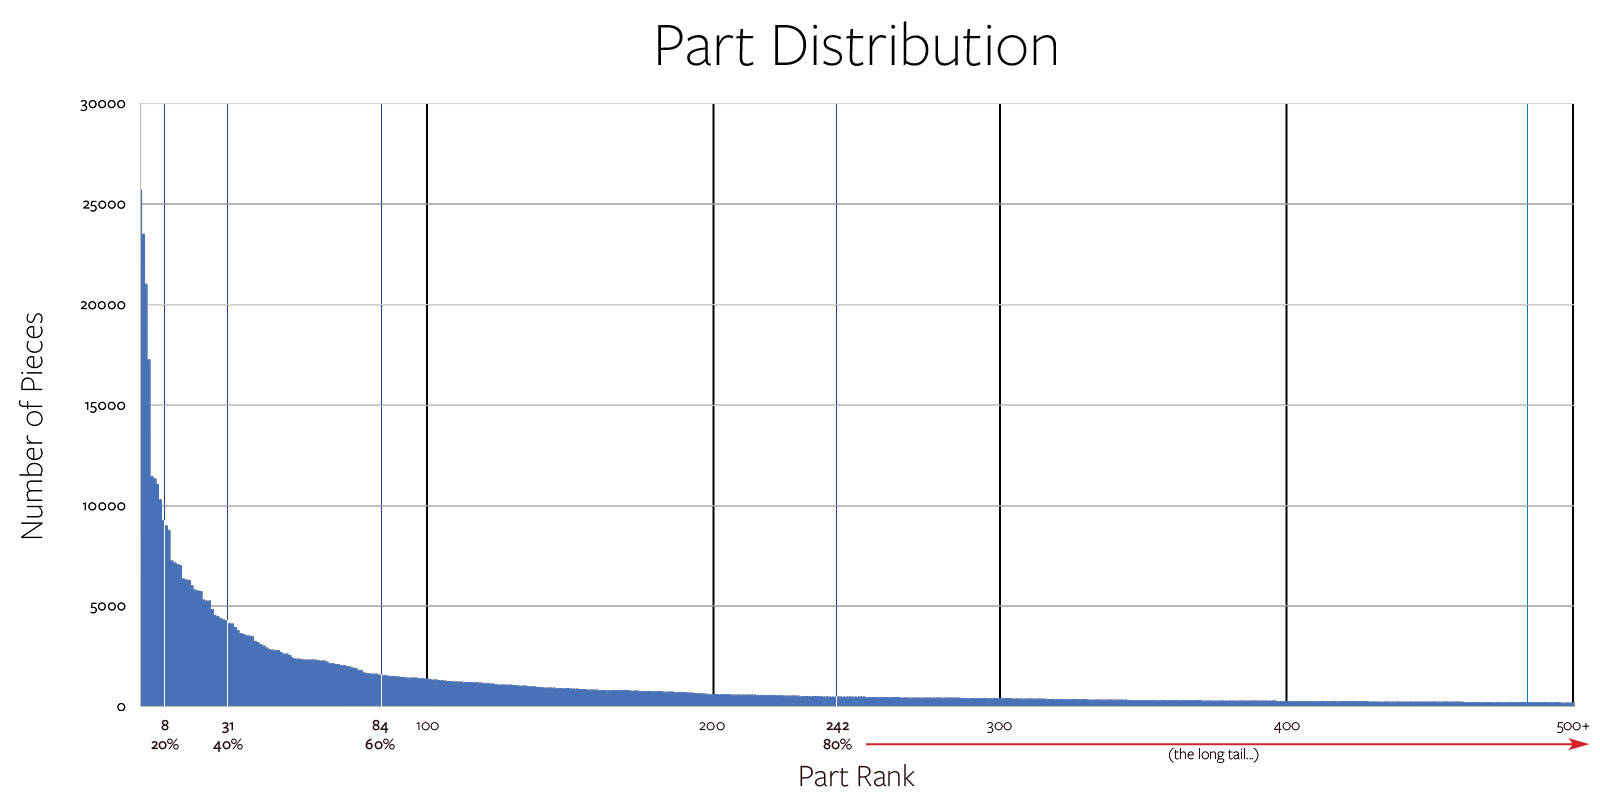
\includegraphics[width=1\textwidth]{images/part_dist.jpg}
%     \caption{Szacunkowa dystrybucja klas klocków kupionych w latach 2015-2020\cite{dist}}
%     \label{fig:part_dist}
% \end{figure}
% Na wykresie \ref{fig:part_dist} terefere.
\section{Cel pracy}
Mój super cel. 
\section{Układ pracy}
Układ pracy jest następujący...


\chapter{WPROWADZENIE DO DZIEDZINY}

To jest rozdział.

\section{Podrozdziały}

W Latexu w klasie dokumentów \textbf{book} wyróżniamy rozdziały (\textbf{chapter}), podrozdziały \textbf{section}, podpodrozdziały \textbf{subsection}, podpodpodrozdziały \textbf{subsubsection} i paragrafy (\textbf{paragraph}). Podpodpodrozdziały i paragrafy domyślnie nie są numerowane ani nie występują w spisie treści. Zachowanie to można zmienić poprzez funkcję \textbf{setcounter} umieszczaną w preambule. Wykomentowany przykład można znaleźć w kodzie tego dokumentu.

Obecnie znajdujemy się na poziomie podrozdziału. Pozostałe przykłady poniżej.

\subsection{Podpodrozdział}

To jest podpodrozdział.

\subsubsection{Podpodpodrozdział}

To jest podpodpodrozdział. On nie jest domyślnie numerowany i nie występuje w spisie treści.

\paragraph{Paragraf}

A to jest paragraf. On również nie jest domyślnie numerowany i nie występuje w spisie treści.

\section{Podstawowe elementy typograficzne}

\subsection{Twarda spacja}

Twarda spacja jest bardzo istotnym elementem, gdyż zabrania Latex'owi łamanie linii w miejscu jej wystąpienia, a tym samym pozwoli na niejako ,,sklejenie'' wyrazów ze sobą. Dzięki temu możemy uniknąć tzw.\ sierot (pojedynczych znaków na końcu wiersza). W Latex twardą spację umieszcza się wstawiając znak tyldy~(\textasciitilde). Zapisujemy to więc np.\ tak: ,,dokument, w{\textasciitilde}którym''.

\subsection{Formatowanie tekstu}

Aby zapewnić poprawny wygląd tekstu należy pamiętać o kilku rzeczach:

\begin{itemize}
 \item Linia poprzedzona procentem to komentarz.
 \item Poprzedzaniu spacji występującej po kropce kończącej skrót znakiem ucieczki, odstęp będzie wtedy taki, jak odstęp między wyrazami a~nie między zdaniami. Przykładowo zapis ,,np. tekst'' vs. ,,np.\ tekst''. Ten drugi jest poprawny, a zapisany został tak: ,,np.$\backslash$~tekst''.
 \item Skróty pisane wielkimi literami kończące zdanie powinny posiadać {$\backslash$}@ przed kropką kończącą zdanie, np.\ OCS{$\backslash$}@\@. Spowoduje to potraktowanie spacji jako spacji międzyzdaniowej z nie międzywyrazowej.
 \item Cudzysłowie zawsze tworzymy używając podwójnego przecinka jako symbolu otwierającego cudzysłów, oraz podwójnego apostrofu zamykającego cudzysłów.
 \item Kursywę uzyskujemy za pomocą słowa kluczowego {$\backslash$}textit, co w efekcie daje \textit{tekst kursywą}. Pogrubiony \textbf{używamy słowa kluczowego textbf}. Każdorazowo tekst mający być napisany danym krojem otaczamy nawiasami klamrowymi.
 \item Myślnik (--) tworzymy poprzez umieszczenie bezpośrednio po sobie dwu kresek (minusy). Różnica między nimi jest zasadnicza. Pojedynczy myślnik generuje krótką kreskę (-), podwójny długą (--), potrójny najdłuższą (---).
 \item Odwołania do różnych elementów dokumentu robimy poprzez słowo kluczowe \textbf{ref()}. Jako jego parametr wstawiamy nazwę zdefiniowaną za pomocą słowa kluczowego \textbf{label()}. Należy pamiętać, że odwołanie zwraca jedynie numer elementu, słowo opisowe, jak np.\ rozdział czy rysunek należy dodać samodzielnie. Polecam tutaj przyjąć jakąś konwencję i się jej trzymać w całym dokumencie. Tak samo należy postępować w przypadku etykiet.
 \item Latex doskonale radzi sobie z dzieleniem wyrazów na końcach linii, jednak czasami zachodzi konieczność wymuszenia podziału w określonym miejscu. W tym celu należy zastosować konstrukcję $\backslash$-. Latex takiego ukośnika nie wydrukuje dopóty, dopóki rzeczywiście w tym miejscu nie zostanie wykonane przeniesienie części wyrazu. Możliwe jest dodanie wielu podziałów w jednym wyrazie. Użyte wtedy zostanie to, które spowoduje wygenerowania ,,najładniejszego'' tekstu.
\end{itemize}

\section{Podział linii i paragrafy}
\label{podzial}

Nowy paragraf rozpoczyna się poprzez wstawienie jednej wolnej linii. Latex automatycznie wygeneruje wcięcie. Należy pamiętać, że pierwszy paragraf, zgodnie ze standardami drukarskimi, nie ma wcięcia! Możemy tym sterować za pomocą poleceń \textbf{noindent} (brak wcięcia) oraz \textbf{indent} (dodatkowe wcięcie).

Jeżeli chcemy po prostu zrobić nową linię, bez tworzenia nowego paragrafu używamy konstrukcji $\backslash\backslash$. Efekt będzie taki, że paragraf\\
będzie kontynuowany w nowej linii. Nie spowoduje to jednak rozciągnięcia poprzedniej linii. Zostanie ona przerwana tam gdzie tego sobie zażyczymy i kontynuowana w nowej linijce.

A co w przypadku, gdy chcemy z jakiegoś powodu przerwać linię, ale wymusić justowanie tekstu? Weźmy dla przykładu fragment:

Trzecim istotnym aspektem jest stosowana w~trakcie wytwarzania ontologii metodologia pracy~\cite{boinski2012kaskbook,boinski2011security}. Zastosowanie jednej z~uznawanych metodologii, takich jak Methontology, NeOn czy metodologia opracowana przez Noy~i~McGuiness, znacząco wpływa na jakoś uzyskanego produktu. Wspomniane metodologie w~dużej mierze uwzględniają potrzebę przyszłej integracji wiedzy, a~w połączeniu z~narzędziami typu Protégé czy OCS~\cite{boinski2007kaskbook,boinski2009ocs,boinski2010zespolowa}, pozwalają na tworzenie spójnych i~formalnie oraz logicznie poprawnych ontologii.

Tekst zostaje bardzo brzydko złamany w środku odnośników do cytowań. Użycie podwójnego po słowie ,,metodologia'' w pierwszym zdaniu ukośnika da nam natomiast taki efekt:

Trzecim istotnym aspektem jest stosowana w~trakcie wytwarzania ontologii metodologia \\ pracy~\cite{boinski2012kaskbook,boinski2011security}. Zastosowanie jednej z~uznawanych metodologii, takich jak Methontology, NeOn czy metodologia opracowana przez Noy~i~McGuiness, znacząco wpływa na jakoś uzyskanego produktu. Wspomniane metodologie w~dużej mierze uwzględniają potrzebę przyszłej integracji wiedzy, a~w połączeniu z~narzędziami typu Protégé czy OCS~\cite{boinski2007kaskbook,boinski2009ocs,boinski2010zespolowa}, pozwalają na tworzenie spójnych i~formalnie oraz logicznie poprawnych ontologii.

Też nie ładnie, gdyż linijka jest niewyjustowana. Z pomocą przychodzi nam tutaj komenda \textbf{linebreak[]}, gdzie w nawiasie kwadratowym podajemy liczbę od 1 do 4 określająca jak bardzo zależy nam na tym, by linia została złamana w tym miejscu (4 to najwyższa wartość). Efekt jest następujący:

Trzecim istotnym aspektem jest stosowana w~trakcie wytwarzania ontologii metodologia \linebreak[4] pracy ~\cite{boinski2012kaskbook,boinski2011security}. Zastosowanie jednej z~uznawanych metodologii, takich jak Methontology, NeOn czy metodologia opracowana przez Noy~i~McGuiness, znacząco wpływa na jakoś uzyskanego produktu. Wspomniane metodologie w~dużej mierze uwzględniają potrzebę przyszłej integracji wiedzy, a~w połączeniu z~narzędziami typu Protégé czy OCS~\cite{boinski2007kaskbook,boinski2009ocs,boinski2010zespolowa}, pozwalają na tworzenie spójnych i~formalnie oraz logicznie poprawnych ontologii.

Jeżeli z jakiegoś powodu potrzebujemy nową linię to używamy komendy \textbf{newpage}. \newpage Tekst występujący po niej znajdzie się na nowej stronie. Rozdziały itp.\ automatycznie generują nową stronę, przy czym w układzie dwustronnym nowy rozdział zawsze zacznie się od nieparzystej strony.

\section{Środowisko matematyczne}

Środowisko matematyczne otwieramy i zamykamy znakiem \$. Niektóre funkcje można używać tylko wewnątrz takiego środowiska. Przykładem niech będzie funkcja \textbf{mathcal} zamieniająca duże litery w symbole o charakterystycznym kroju, stosowanym do opisywania stałych, np.\ $\mathcal{O}$ czy $\mathcal{R(D,P,T,S,U,I)}$. Pamiętać należy, że zamienione zostaną wszystkie litery w wyrażeniu występującym wewnątrz nawiasów klamrowych.

Niektóre konstrukcje, np.\ równania, automatycznie włączają tryb matematyczny. Równania dobrze jest opisać, przykład przedstawia Równanie~\ref{eq:przyklad}.

\begin{equation}
  \mathcal{O(K,B,C,R)}
  \label{eq:przyklad}
\end{equation}

gdzie:\\
$\mathcal{K}$ - zbiór klas wchodzących w~skład ontologii,\\
$\mathcal{B}$ - zbiór bytów wchodzących w~skład ontologii,\\
$\mathcal{C}$ - zbiór komentarzy przypisanych do klas $\mathcal{K}$ i~bytów $\mathcal{B}$ wchodzących w~skład ontologii,\\
$\mathcal{R}$ - zbiór relacji wiążących elementy ontologii.


W równaniach możemy stosować różne dodatkowe symbole oraz np.\ wyrównywać je do określonego miejsca. Służy do tego blok typu \textbf{split}, a sam punkt wyrównania określony jest ampersandem (\&). Przykład zastosowania prezentuje równanie~\ref{eq:split_ex}.

\begin{equation}
  \label{eq:split_ex}
  \begin{split}
    \forall {x_1 \leq y_1, x_2 \leq y_2}&: f(x_1+x_2,y_1+y_2)\\ 
				  &= \frac{y_1}{y_1+y_2}f(x_1,y_1)+\frac{y_2}{y_1+y_2}f(x_2,y_2)
  \end{split}
\end{equation}

\subsection{Twierdzenia i dowody}

Linie 75 -- 93 nagłówka dokumentu definiują nowe nazwy sekcji twierdzeń i dowodów, oraz znacznik końca dowodu (taki czarny kwadracik). Dzięki nim można uzyskać ładnie wyglądające twierdzenia jak poniżej (Twierdzenie~\ref{eq:lin:theorem}). Zauważmy, że równanie dowodu nie jest równaniem numerowanym. Wszędzie tam, gdzie nie chcemy by rozdział czy dowolna inna sekcja była numerowana należy w jej nazwie użyć gwiazdki, np. \textbf{$\backslash$begin\{equation*\}}.

\begin{theorem}
 Podobieństwo pomiędzy pojęciami $A$ i~$B$ opisane jest stosunkiem ilości informacji niezbędnej do opisania ich wspólności znaczeniowej oraz ilością informacji niezbędnej do ich opisania (Równanie~\ref{eq:lin:theoremeq}).

 \begin{equation}
   sim_{lin}(A,B)=\frac{\log P(common(A,B))}{\log P(description(A,B))}
   \label{eq:lin:theoremeq}
 \end{equation}
 \label{eq:lin:theorem}
\end{theorem}

\begin{proof}
  \begin{equation*}
   \begin{split}
     f(x,y)&=f(x+0,y+(y-x))\\
	   &=\frac{x}{y}*f(x,x) +~\frac{y-z}{x}*f(0,y-z)\\
	   &=\frac{x}{y}*1 +~\frac{y-z}{x}*0\\
	   &=\frac{x}{y} \qed
   \end{split}
 \end{equation*}
\end{proof}

Inna ciekawa konstrukcja wykorzystująca tryb matematyczny do zapisania pewnego stwierdzenia:

Niech $A \subseteq T$, $C = N_y(A) \neq W$, a~$\alpha_y = \min_{a \in A, b\notin C} \{y(a) +~y(b) - q(a, b)\}$ oraz

\[ y'(v) = \left\{ \begin{array}{ll}
                y(v) - \alpha_y & \mbox{jeżeli $v \in A$} \\
                y(v) +~\alpha_y & \mbox{jeżeli $v \in C$} \\
                y(v)            & \mbox{w innych przypadkach}
               \end{array}
       \right. \]

Zapis ten, acz skomplikowany, pozwala na reprezentację złożonych reguł matematycznych w postaci ładnie ułożonych i wyrównanych wierszy. Reguły \textbf{left} oraz \textbf{right} pozwalają na utworzenie nawiasów klamrowych, których rozmiar będzie automatycznie dostosowywany do rozmiaru elementu, jakie mają zawierać.

\chapter{TECHNOLOGIE, ALGORYTMY I NARZĘDZIA}

To jest rozdział.

\section{Podrozdziały}

W Latexu w klasie dokumentów \textbf{book} wyróżniamy rozdziały (\textbf{chapter}), podrozdziały \textbf{section}, podpodrozdziały \textbf{subsection}, podpodpodrozdziały \textbf{subsubsection} i paragrafy (\textbf{paragraph}). Podpodpodrozdziały i paragrafy domyślnie nie są numerowane ani nie występują w spisie treści. Zachowanie to można zmienić poprzez funkcję \textbf{setcounter} umieszczaną w preambule. Wykomentowany przykład można znaleźć w kodzie tego dokumentu.

Obecnie znajdujemy się na poziomie podrozdziału. Pozostałe przykłady poniżej.

\subsection{Podpodrozdział}

To jest podpodrozdział.

\subsubsection{Podpodpodrozdział}

To jest podpodpodrozdział. On nie jest domyślnie numerowany i nie występuje w spisie treści.

\paragraph{Paragraf}

A to jest paragraf. On również nie jest domyślnie numerowany i nie występuje w spisie treści.


\chapter{PROJEKT SYSTEMU}

tekst, tu już typowo o naszej implementacji (porównywać do papieru), na początku krótki opis że dzieli sie na front i backend i model


\section{Interfejs gry \textit{Kacper Konopka}}

% cały opis unity, za co odpowiada, jakie są interakcje, animacje
Aby przedstawić świat, w którym operują agenci stworzone zostały interfejsy ułatwiające interpretacje przez człowieka. Dzięki nim osoba uczestnicząca jest w stanie zaobserwować zachowania agentów jako grę. Do stworzenia takiego środowiska użyto silnik do gier Unity, który zawiera wiele elementów interaktywnych pozwalających zarówno tworzyć agentów jak i zobaczyć ich aktualny stan. Oprócz części, w których obserwator może wpływać na środowisko są również te, które prezentują elementy otoczenia np. drzewa, domy bądź rzeki.

\subsection{Elementy interaktywne}
Celem stworzenia imersji obserwator ma możliwość ingerowania w świat agentów poprzez następujące elementy.
\subsubsection{Interfejs tworzenia nowych agentów}
W ramach udostęnienia możliwości tworzenia nowych agentów stworzono okno, w którym użytkownik wprowadza informacje na temat agenta. Każde z pól - imię (ang. \textit{Name}), wiek (ang. \textit{Age}), opis agenta (ang. \textit{Description}) oraz styl życia (ang. \textit{Lifestyle}) musi zostać wypełnione aby agenta stworzyć. W przeciwnym przypadku przy naciśnięciu przycisku \textit{Submit} gra poinformuje nas o tym, że jedno z tych pól jest puste a agent nie zostanie stworzony. Oprócz wypełnienia informacji tekstowych możemy również wybrać wygląd agenta spośród uprzednio stworzonych zasobów. Gdy użytkownik nie wybierze modelu postaci, dobierany jest pierwszy zasób z listy. Aby zakończyć tworzenie agenta użytkownik musi nacisnąć przycisk \textit{Submit}. Gdy wszystkie wyżej wymienione warunki są spełnione agent pojawia się na środku mapy.
Wypełniony interfejs prezentuje rysunek~\ref{fig:createagent}.
\begin{figure}[htbp]
    \centering
    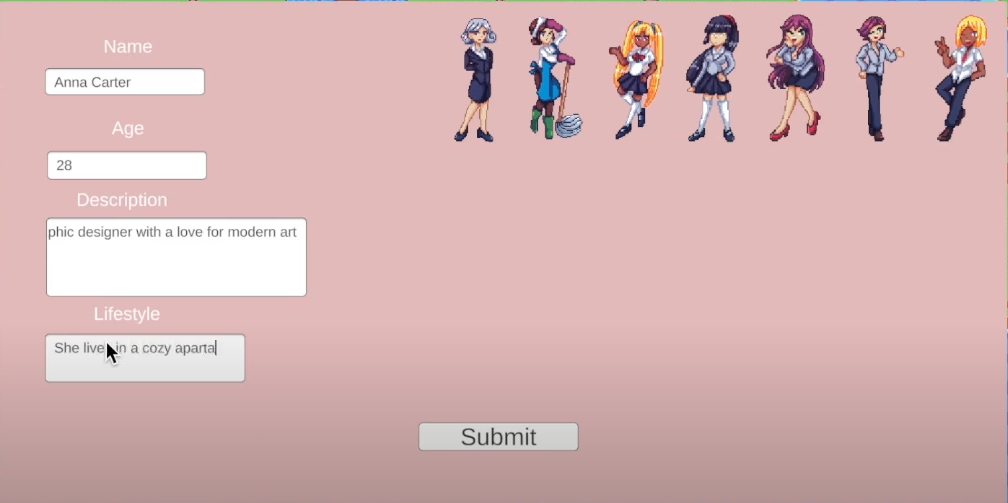
\includegraphics[width=0.9\textwidth]{images/411.png}
    \caption{Rysunek przedstawiający przykładowy, prawidłowo wypełniony interfejs tworzenia agenta.}
    \label{fig:createagent}
\end{figure}
\subsubsection{Interfejs stanu agenta}
Ważnym elementem obserwacji działania agentów jest wyświetlanie ich stanu. W tym celu stworzono interfejs, który wyświetla podstawowe informacje o agencie. Aby uzyskać informacje o agencie należy kliknąć na agenta, który znajduje się w polu widzenia. W skład danych, które znajdują się w oknie znajdują się elementy takie jak - aktualna data i godzina wydarzeń, identyfikator agenta, imię (ang. \textit{Name}), wiek (ang. \textit{Age}), opis agenta (ang. \textit{Description}) oraz styl życia (ang. \textit{Lifestyle}). Przrykładowy stan agenta ukazany jest w rysunku~\ref{fig:stateagent}. Okno interfejsu stanu agenta jest półprzezroczyste, przez co można zauważyć niektóre elementy środowiska, które nie przeszkadzają w interpretacji przedstawionych danych.
\begin{figure}[htbp]
    \centering
    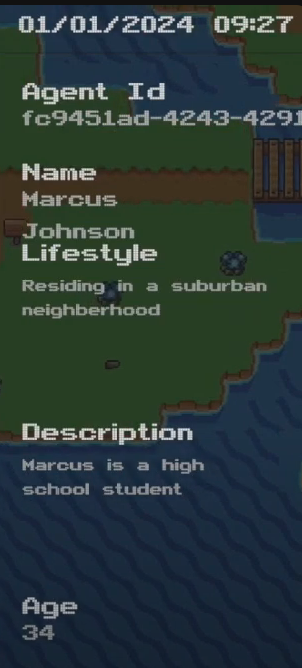
\includegraphics[width=0.9\textwidth, height=0.6\textheight]{images/411state.png}
    \caption{Rysunek przedstawiający przykładowy interfejs stanu agenta.}
    \label{fig:stateagent}
\end{figure}


\section{Architektura serwera i warstwy logicznej}
\label{sec:architektura_serwera}

\subsection{Agenci}

\subsubsection{Pamięć agentów}
Pamięć agentów jest kluczowym elementem ich funkcjonowania.
To dzięki niej agenci reagują w sposób bardziej ludzki.

\paragraph{Architektura pamięci agentów}
Pamięć opiera się na modelu języka naturalnego typu encoder, który przekształca
nowe wspomnienia agenta na wektor. Później, w trakcie interakcji czy budowania nowych
wspomnień przez agenta jest wybierane k wspomnień, które uzyskały największą średnią
ważoną z trzech metryk: podobieństwa (relevance), ważności (importance) i niedawności (recency).
Wybrane wspomnienia są później przekazywane do modelu językowego typu decoder, który na
podstawie ich i danego wydarzenia decyduje o zachowaniu agenta.

\paragraph{Metryka podobieństwa}
Metryka podobieństwa odpowiada podobieństwu tematycznemu nowego wydarzenia do
wydarzenia zapisanego w pamięci agenta. Jest to uzyskiwane za pomocą obliczonej
odległości cosinusowej wektorów stworzonych przez model typu encoder.

\paragraph{Metryka ważności}
Metryka istoty jest uzyskiwana
poprzez ocenę ważności danego wydarzenia w kontekście życia agenta przez LLM.
Metryka odpowiada na pytanie jak ważne dla danego agenta w skali od 1 do 10 jest
dane wydarzenie np. pościelenie łóżka będzie miało skalę bliską 1, gdzie wzięcie
ślubu skalę bliską 10.

\paragraph{Metryka niedawności}
Metryka niedawności odpowiada mechanizmowi "zapominania" przez agenta.
Wspomnienia uzyskują wynik zgodnie ze wzorem:

\begin{equation}
 \label{eq:metryka_niedawnosci}
	score = max\_score * decay\_factor ^ {time\_diff}
\end{equation}




\section{Polecenia dla modeli językowych}

% przenieść do teorii 
Jakość odpowiedzi generowanych przez duże modele językowe w znacznym stopniu zależy od~zapytań, które są do nich wysyłane. Tekst przekazywany do modelu nazywany jest poleceniem (ang. \textit{prompt}), którego główną częścią jest pytanie lub zadanie opisujące, co model powinien wykonać. W przypadku techniki RAG w skład polecenia wchodzi także kontekst, czyli tekst ukazujący szerszą perspektywę danego tematu. W~samym zadaniu zawarta jest także informacja dla modelu, aby ten, podczas odpowiadania na pytanie lub wykonywania postawionego mu zadania, korzystał bezpośrednio z dostarczonego mu kontekstu - jeżeli jakaś informacja w nim nie występuje, model powinien jasno zakomunikować, że nie jest w stanie odpowiedzieć na pytanie. Nie powinien próbować wymyślać odpowiedzi jedynie na podstawie własnej wiedzy.

\subsection{Wykonywanie akcji}

W aplikacji SMIS, podobnie jak w programie, na którym wzorowana jest jej implementacja~\cite{park2023generativeagentsinteractivesimulacra}, każda decyzja dotycząca przebiegu rozgrywki podejmowana jest za pomocą dużego modelu językowego. W~ujęciu ogólnym, na podstawie otrzymanych odpowiedzi, wykonywane są odpowiednie akcje. Kiedy rozpoczyna się dzień, dla każdego agenta generowany jest godzinowy plan dnia, bazujący na~jego zainteresowaniach i jego trybie życia. Agent przeżywa dzień zgodnie z tym planem. Ponadto, przy~każdym spotkaniu z inną osobą, model językowy decyduje, czy agenci powinni nawiązać konwersację. Jeśli decyzja jest pozytywna, tworzona jest konwersacja, która nawiązuje do~wspomnień rozmówców oraz jest zgodna z~ich osobowościami. Po zakończeniu rozmowy jest ona podsumowywana i generowane są wspomnienia dla obu agentów, które zapisywane są w~ich pamięci. Dzięki temu mogą się oni do nich odwoływać w odpowiednich do tego momentach.

Przy tworzeniu polecenia dla modelu, pobierane są informacje i wspomnienia odnoszące się do~konkretnego agenta. Żeby proces ten mógł nastąpić, należy podczas zapisywania wspomnienia uwzględnić trzy metryki, opisane szerzej w podrozdziale \ref{sec:architektura_serwera}. Metryka ważności również opiera się na odpowiedzi od modelu.

\subsection{Konwersacje}

Tworzenie konwersacji jest dość skomplikowanym procesem. Aby jak najbardziej upodobnić agentów do prawdziwych ludzi, generowanie rozmowy podzielone zostało na kilka etapów.

Pierwszym z nich jest decydowanie, czy agent powinien w ogóle podjąć konwersację. Warto zauważyć, że my również nie odzywamy się do każdej miniętej na ulicy osoby - w takiej sytuacji nie udawałoby nam się nigdzie dotrzeć, gdyż cały dzień wypełniony byłby jedynie rozmowami z innymi. Podświadomie oceniamy, czy warto przywitać się z daną osobą. Czynniki, jakie są w takiej sytuacji brane pod uwagę, to m.in. to, kim jest spotkany człowiek, czy go znamy, co w danym momencie robi, czy nie jest zajęty.

Podobnie działają agenci w aplikacji SMIS.




\section{Komunikacja między serwisami}

jak jest zrobiona komunikacja, jak to działa, może być wiele frontów na jeden serwer

\chapter{BADANIA}

To jest rozdział.

\section{Podrozdziały}

W Latexu w klasie dokumentów \textbf{book} wyróżniamy rozdziały (\textbf{chapter}), podrozdziały \textbf{section}, podpodrozdziały \textbf{subsection}, podpodpodrozdziały \textbf{subsubsection} i paragrafy (\textbf{paragraph}). Podpodpodrozdziały i paragrafy domyślnie nie są numerowane ani nie występują w spisie treści. Zachowanie to można zmienić poprzez funkcję \textbf{setcounter} umieszczaną w preambule. Wykomentowany przykład można znaleźć w kodzie tego dokumentu.

Obecnie znajdujemy się na poziomie podrozdziału. Pozostałe przykłady poniżej.

\subsection{Podpodrozdział}

To jest podpodrozdział.

\subsubsection{Podpodpodrozdział}

To jest podpodpodrozdział. On nie jest domyślnie numerowany i nie występuje w spisie treści.

\paragraph{Paragraf}

A to jest paragraf. On również nie jest domyślnie numerowany i nie występuje w spisie treści.

\section{Podstawowe elementy typograficzne}

\subsection{Twarda spacja}

Twarda spacja jest bardzo istotnym elementem, gdyż zabrania Latex'owi łamanie linii w miejscu jej wystąpienia, a tym samym pozwoli na niejako ,,sklejenie'' wyrazów ze sobą. Dzięki temu możemy uniknąć tzw.\ sierot (pojedynczych znaków na końcu wiersza). W Latex twardą spację umieszcza się wstawiając znak tyldy~(\textasciitilde). Zapisujemy to więc np.\ tak: ,,dokument, w{\textasciitilde}którym''.

\subsection{Formatowanie tekstu}

Aby zapewnić poprawny wygląd tekstu należy pamiętać o kilku rzeczach:

\begin{itemize}
 \item Linia poprzedzona procentem to komentarz.
 \item Poprzedzaniu spacji występującej po kropce kończącej skrót znakiem ucieczki, odstęp będzie wtedy taki, jak odstęp między wyrazami a~nie między zdaniami. Przykładowo zapis ,,np. tekst'' vs. ,,np.\ tekst''. Ten drugi jest poprawny, a zapisany został tak: ,,np.$\backslash$~tekst''.
 \item Skróty pisane wielkimi literami kończące zdanie powinny posiadać {$\backslash$}@ przed kropką kończącą zdanie, np.\ OCS{$\backslash$}@\@. Spowoduje to potraktowanie spacji jako spacji międzyzdaniowej z nie międzywyrazowej.
 \item Cudzysłowie zawsze tworzymy używając podwójnego przecinka jako symbolu otwierającego cudzysłów, oraz podwójnego apostrofu zamykającego cudzysłów.
 \item Kursywę uzyskujemy za pomocą słowa kluczowego {$\backslash$}textit, co w efekcie daje \textit{tekst kursywą}. Pogrubiony \textbf{używamy słowa kluczowego textbf}. Każdorazowo tekst mający być napisany danym krojem otaczamy nawiasami klamrowymi.
 \item Myślnik (--) tworzymy poprzez umieszczenie bezpośrednio po sobie dwu kresek (minusy). Różnica między nimi jest zasadnicza. Pojedynczy myślnik generuje krótką kreskę (-), podwójny długą (--), potrójny najdłuższą (---).
 \item Odwołania do różnych elementów dokumentu robimy poprzez słowo kluczowe \textbf{ref()}. Jako jego parametr wstawiamy nazwę zdefiniowaną za pomocą słowa kluczowego \textbf{label()}. Należy pamiętać, że odwołanie zwraca jedynie numer elementu, słowo opisowe, jak np.\ rozdział czy rysunek należy dodać samodzielnie. Polecam tutaj przyjąć jakąś konwencję i się jej trzymać w całym dokumencie. Tak samo należy postępować w przypadku etykiet.
 \item Latex doskonale radzi sobie z dzieleniem wyrazów na końcach linii, jednak czasami zachodzi konieczność wymuszenia podziału w określonym miejscu. W tym celu należy zastosować konstrukcję $\backslash$-. Latex takiego ukośnika nie wydrukuje dopóty, dopóki rzeczywiście w tym miejscu nie zostanie wykonane przeniesienie części wyrazu. Możliwe jest dodanie wielu podziałów w jednym wyrazie. Użyte wtedy zostanie to, które spowoduje wygenerowania ,,najładniejszego'' tekstu.
\end{itemize}

\section{Podział linii i paragrafy}
\label{podzial}

Nowy paragraf rozpoczyna się poprzez wstawienie jednej wolnej linii. Latex automatycznie wygeneruje wcięcie. Należy pamiętać, że pierwszy paragraf, zgodnie ze standardami drukarskimi, nie ma wcięcia! Możemy tym sterować za pomocą poleceń \textbf{noindent} (brak wcięcia) oraz \textbf{indent} (dodatkowe wcięcie).

Jeżeli chcemy po prostu zrobić nową linię, bez tworzenia nowego paragrafu używamy konstrukcji $\backslash\backslash$. Efekt będzie taki, że paragraf\\
będzie kontynuowany w nowej linii. Nie spowoduje to jednak rozciągnięcia poprzedniej linii. Zostanie ona przerwana tam gdzie tego sobie zażyczymy i kontynuowana w nowej linijce.

A co w przypadku, gdy chcemy z jakiegoś powodu przerwać linię, ale wymusić justowanie tekstu? Weźmy dla przykładu fragment:

Trzecim istotnym aspektem jest stosowana w~trakcie wytwarzania ontologii metodologia pracy~\cite{boinski2012kaskbook,boinski2011security}. Zastosowanie jednej z~uznawanych metodologii, takich jak Methontology, NeOn czy metodologia opracowana przez Noy~i~McGuiness, znacząco wpływa na jakoś uzyskanego produktu. Wspomniane metodologie w~dużej mierze uwzględniają potrzebę przyszłej integracji wiedzy, a~w połączeniu z~narzędziami typu Protégé czy OCS~\cite{boinski2007kaskbook,boinski2009ocs,boinski2010zespolowa}, pozwalają na tworzenie spójnych i~formalnie oraz logicznie poprawnych ontologii.

Tekst zostaje bardzo brzydko złamany w środku odnośników do cytowań. Użycie podwójnego po słowie ,,metodologia'' w pierwszym zdaniu ukośnika da nam natomiast taki efekt:

Trzecim istotnym aspektem jest stosowana w~trakcie wytwarzania ontologii metodologia \\ pracy~\cite{boinski2012kaskbook,boinski2011security}. Zastosowanie jednej z~uznawanych metodologii, takich jak Methontology, NeOn czy metodologia opracowana przez Noy~i~McGuiness, znacząco wpływa na jakoś uzyskanego produktu. Wspomniane metodologie w~dużej mierze uwzględniają potrzebę przyszłej integracji wiedzy, a~w połączeniu z~narzędziami typu Protégé czy OCS~\cite{boinski2007kaskbook,boinski2009ocs,boinski2010zespolowa}, pozwalają na tworzenie spójnych i~formalnie oraz logicznie poprawnych ontologii.

Też nie ładnie, gdyż linijka jest niewyjustowana. Z pomocą przychodzi nam tutaj komenda \textbf{linebreak[]}, gdzie w nawiasie kwadratowym podajemy liczbę od 1 do 4 określająca jak bardzo zależy nam na tym, by linia została złamana w tym miejscu (4 to najwyższa wartość). Efekt jest następujący:

Trzecim istotnym aspektem jest stosowana w~trakcie wytwarzania ontologii metodologia \linebreak[4] pracy~\cite{boinski2012kaskbook,boinski2011security}. Zastosowanie jednej z~uznawanych metodologii, takich jak Methontology, NeOn czy metodologia opracowana przez Noy~i~McGuiness, znacząco wpływa na jakoś uzyskanego produktu. Wspomniane metodologie w~dużej mierze uwzględniają potrzebę przyszłej integracji wiedzy, a~w połączeniu z~narzędziami typu Protégé czy OCS~\cite{boinski2007kaskbook,boinski2009ocs,boinski2010zespolowa}, pozwalają na tworzenie spójnych i~formalnie oraz logicznie poprawnych ontologii.

Jeżeli z jakiegoś powodu potrzebujemy nową linię to używamy komendy \textbf{newpage}. \newpage Tekst występujący po niej znajdzie się na nowej stronie. Rozdziały itp.\ automatycznie generują nową stronę, przy czym w układzie dwustronnym nowy rozdział zawsze zacznie się od nieparzystej strony.

\section{Środowisko matematyczne}

Środowisko matematyczne otwieramy i zamykamy znakiem \$. Niektóre funkcje można używać tylko wewnątrz takiego środowiska. Przykładem niech będzie funkcja \textbf{mathcal} zamieniająca duże litery w symbole o charakterystycznym kroju, stosowanym do opisywania stałych, np.\ $\mathcal{O}$ czy $\mathcal{R(D,P,T,S,U,I)}$. Pamiętać należy, że zamienione zostaną wszystkie litery w wyrażeniu występującym wewnątrz nawiasów klamrowych.

Niektóre konstrukcje, np.\ równania, automatycznie włączają tryb matematyczny. Równania dobrze jest opisać, przykład przedstawia Równanie~\ref{eq:przyklad}.

\begin{equation}
  \mathcal{O(K,B,C,R)}
  \label{eq:przyklad}
\end{equation}

gdzie:\\
$\mathcal{K}$ - zbiór klas wchodzących w~skład ontologii,\\
$\mathcal{B}$ - zbiór bytów wchodzących w~skład ontologii,\\
$\mathcal{C}$ - zbiór komentarzy przypisanych do klas $\mathcal{K}$ i~bytów $\mathcal{B}$ wchodzących w~skład ontologii,\\
$\mathcal{R}$ - zbiór relacji wiążących elementy ontologii.


W równaniach możemy stosować różne dodatkowe symbole oraz np.\ wyrównywać je do określonego miejsca. Służy do tego blok typu \textbf{split}, a sam punkt wyrównania określony jest ampersandem (\&). Przykład zastosowania prezentuje równanie~\ref{eq:split_ex}.

\begin{equation}
  \label{eq:split_ex}
  \begin{split}
    \forall {x_1 \leq y_1, x_2 \leq y_2}&: f(x_1+x_2,y_1+y_2)\\ 
				  &= \frac{y_1}{y_1+y_2}f(x_1,y_1)+\frac{y_2}{y_1+y_2}f(x_2,y_2)
  \end{split}
\end{equation}

\subsection{Twierdzenia i dowody}

Linie 75 -- 93 nagłówka dokumentu definiują nowe nazwy sekcji twierdzeń i dowodów, oraz znacznik końca dowodu (taki czarny kwadracik). Dzięki nim można uzyskać ładnie wyglądające twierdzenia jak poniżej (Twierdzenie~\ref{eq:lin:theorem}). Zauważmy, że równanie dowodu nie jest równaniem numerowanym. Wszędzie tam, gdzie nie chcemy by rozdział czy dowolna inna sekcja była numerowana należy w jej nazwie użyć gwiazdki, np. \textbf{$\backslash$begin\{equation*\}}.

\begin{theorem}
 Podobieństwo pomiędzy pojęciami $A$ i~$B$ opisane jest stosunkiem ilości informacji niezbędnej do opisania ich wspólności znaczeniowej oraz ilością informacji niezbędnej do ich opisania (Równanie~\ref{eq:lin:theoremeq}).

 \begin{equation}
   sim_{lin}(A,B)=\frac{\log P(common(A,B))}{\log P(description(A,B))}
   \label{eq:lin:theoremeq}
 \end{equation}
 \label{eq:lin:theorem}
\end{theorem}

\begin{proof}
  \begin{equation*}
   \begin{split}
     f(x,y)&=f(x+0,y+(y-x))\\
	   &=\frac{x}{y}*f(x,x) +~\frac{y-z}{x}*f(0,y-z)\\
	   &=\frac{x}{y}*1 +~\frac{y-z}{x}*0\\
	   &=\frac{x}{y} \qed
   \end{split}
 \end{equation*}
\end{proof}

Inna ciekawa konstrukcja wykorzystująca tryb matematyczny do zapisania pewnego stwierdzenia:

Niech $A \subseteq T$, $C = N_y(A) \neq W$, a~$\alpha_y = \min_{a \in A, b\notin C} \{y(a) +~y(b) - q(a, b)\}$ oraz

\[ y'(v) = \left\{ \begin{array}{ll}
                y(v) - \alpha_y & \mbox{jeżeli $v \in A$} \\
                y(v) +~\alpha_y & \mbox{jeżeli $v \in C$} \\
                y(v)            & \mbox{w innych przypadkach}
               \end{array}
       \right. \]

Zapis ten, acz skomplikowany, pozwala na reprezentację złożonych reguł matematycznych w postaci ładnie ułożonych i wyrównanych wierszy. Reguły \textbf{left} oraz \textbf{right} pozwalają na utworzenie nawiasów klamrowych, których rozmiar będzie automatycznie dostosowywany do rozmiaru elementu, jakie mają zawierać.

\chapter{PODSUMOWANIE}
\label{chap:podsumowanie}

tekst

\section{Osiągnięte rezultaty}

tekst

\section{Plany na przyszłość}

tekst


% Bibliografia, ignorujemy overfull box, bo są długie URL
\hfuzz=50pt
\printbibliography[title=\bibliographyname]
\addcontentsline{toc}{chapter}{\bibliographyname}
\hfuzz=0pt

% Wykaz rysunków
\listoffigures
\addcontentsline{toc}{chapter}{\listfigurename}

% Wykaz tabel
\listoftables
\addcontentsline{toc}{chapter}{\listtablename}


\end{document}
